%==============================================================================
% Section 5: Mode Dictionary: Nil^3 x S^1 under EC-Weyl
%==============================================================================
\section{Mode Dictionary: $\Nilthree\times\Sone$ under EC--Weyl}
\label{sec:nil3}

This section analyses in detail the effect of the EC--Weyl coupling on the
homogeneous geometric degrees of freedom of $\Nilthree\times\Sone$.  Among the
three topologies, $\Nilthree$ is the only non-conformally flat manifold, and
this property generates---via the EC--Weyl coupling---an EC false vacuum
(Theorem~6), a spin-2 quintet splitting (Theorem~7), and a uniaxial mass
splitting (Theorem~8), all absent in LC.

\subsection{Geometric Properties of $\Nilthree$}
\label{sec:nil3:geom}

The geometry of $\Nilthree$ (the three-dimensional Heisenberg manifold) is
characterised by a single non-zero structure constant:
\begin{equation}
  C^2_{01}(\Nilthree) = \frac{1}{R},
\end{equation}
where $R$ is the scale parameter of $\Nilthree$.  We adopt the convention
$[E_0,E_1] = (1/R)E_2$.  In the implementation, the Maurer--Cartan form
$\dd\sigma^2 = -\sigma^0\wedge\sigma^1$ is used as the basis, so the frame
coefficient is $C[2,0,1] = -(1+\varepsilon)^{-4/3}(1+s)^{-2}/R$.  Both
expressions describe the same Heisenberg structure and differ only by a
convention choice.  This single-component Lie structure is the source of the
spin-2 quintet splitting and uniaxial mass splitting discussed below.

\paragraph{Non-conformal flatness.}
The background ($\eta=V=0$) Weyl scalar is
\begin{equation}
  C^2_\LC(\Nilthree,\,\eta=V=0) = \frac{4}{3R^4} \neq 0.
\end{equation}
This non-conformal flatness activates the EC--Weyl coupling $\alpha\cdot C^2_\EC$
even on the $\eta=V=0$ section, generating the false vacuum (\S\ref{sec:nil3:fv}).

The auxiliary cubic coefficient satisfies
\begin{equation}
  C_\delta(\Nilthree) = 0,
  \qquad
  \frac{\partial C_\delta(\Nilthree)}{\partial\alpha} = 0
\end{equation}
(Theorem~\ref{thm:delta}, Appendix~\ref{app:D}).  The EC-specific physics of
$\Nilthree$ therefore appears in the background Weyl and the $(r,\eta,V)$
sector, not as a new $\delta$-sector cubic channel.

\subsection{Theorem~6: $\Nilthree$ EC False Vacuum}
\label{sec:nil3:fv}

\begin{theorem}[$\Nilthree$ EC false vacuum]\label{thm:fv}
  For $\alpha<0$, the homogeneous effective potential of $\Nilthree\times\Sone$
  supports a positive false vacuum on the $\eta=V=0$ section\textup{:}
  \begin{equation}
    r_0 = \frac{4\kappa}{\sqrt{3}}\sqrt{|\alpha|},
    \qquad
    V_0 = \frac{32\sqrt{3}\,\pi^4 La}{3\kappa} > 0,
    \quad (\alpha = -a^2,\; a>0).
  \end{equation}
  Here ``false vacuum'' refers to a local minimum of the homogeneous effective
  potential.
\end{theorem}

\begin{proof}
  By AX/VT dropout (Theorem~\ref{thm:dropout}), in the AX background ($V=0$)
  and the VT background ($\eta=0$), $C^2_\EC = C^2_\LC$ holds, so the EC
  extension does not shift the LC stationarity conditions.  (Since
  $C^2_\LC(\Nilthree)\neq 0$, the $\alpha$-dependence through the LC--Weyl term
  remains, but this is already present in LC.)

  On the $\eta=V=0$ isotropic section, SymPy confirms the two-term structure:
  \begin{equation}
    \Veff^{Nil^3}(r,\,\eta=0,\,V=0;\,\alpha,\,\theta=0)
    = \frac{4\pi^4 Lr}{\kappa^2} - \frac{64\pi^4 L\alpha}{3r}.
  \end{equation}
  The first term is the LC contribution (power $n=1$) and the second is the
  EC--Weyl contribution (power $m=-1$).

  The stationarity condition $\partial\Veff/\partial r=0$ gives
  \begin{equation}
    \frac{4\pi^4 L}{\kappa^2} + \frac{64\pi^4 L\alpha}{3r^2} = 0
    \quad\Rightarrow\quad
    r_0^2 = -\frac{16\alpha\kappa^2}{3} = \frac{16|\alpha|\kappa^2}{3},
    \quad
    r_0 = \frac{4\kappa}{\sqrt{3}}\sqrt{|\alpha|}.
  \end{equation}
  The vacuum energy is
  \begin{equation}
    V_0 = \Veff(r_0) = \frac{32\sqrt{3}\,\pi^4 La}{3\kappa} > 0
    \quad (\alpha = -a^2 < 0),
  \end{equation}
  establishing a positive local minimum (false vacuum).
\end{proof}

\paragraph{Numerical verification.}

\begin{table}[H]
\centering
\begin{tabular}{lllllll}
\toprule
$\alpha$ & $r_0$ (analytic) & $r_0$ (numeric) & Error & $V_0$ (analytic) & $V_0$ (numeric) & Error \\
\midrule
$-0.05$ & 0.516398 & 0.516400 & 0.0004\% & 402.415 & 402.415 & $<10^{-6}$\% \\
$-0.50$ & 1.632993 & 1.633000 & 0.0004\% & 1272.547 & 1272.547 & $<10^{-6}$\% \\
$-1.00$ & 2.309401 & 2.309400 & 0.0000\% & 1799.653 & 1799.653 & $<10^{-6}$\% \\
$-3.00$ & 4.000000 & 4.000000 & 0.0000\% & 3117.091 & 3117.091 & 0\% \\
\bottomrule
\end{tabular}
\caption{Analytic vs.\ numeric comparison for the $\Nilthree$ EC false vacuum
  (with $\kappa=L=1$).}
\label{tab:nil3fv}
\end{table}

\begin{figure}[H]
  \centering
  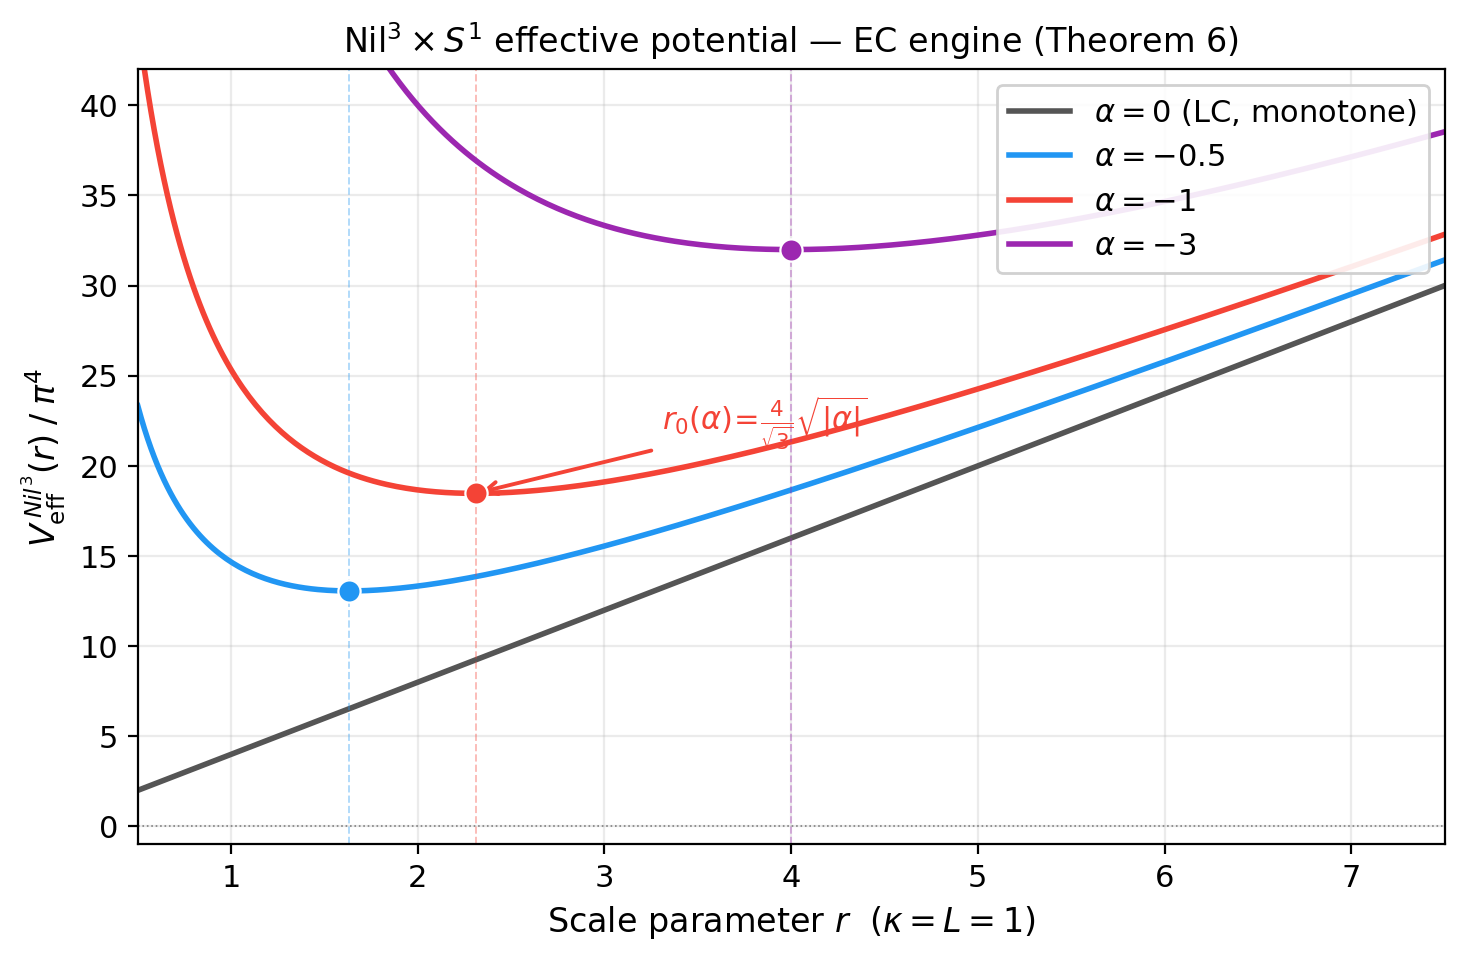
\includegraphics[width=0.9\textwidth]{figures/fig01_nil3_veff.png}
  \caption{$\Nilthree$ effective potential $\Veff(r)$ on the $\eta=V=0$ section
    for $\alpha=-1$, $\kappa=L=1$.  The LC part ($\alpha=0$, dashed) is
    monotonically increasing; the EC--Weyl term ($-64\pi^4 L\alpha/(3r)$)
    creates a local minimum at $r_0 = 2.309$ (false vacuum, solid).}
  \label{fig:nil3veff}
\end{figure}

\subsection{Theorem~7: $\Nilthree$ Spin-2 Quintet Splitting}
\label{sec:nil3:thm7}

\begin{theorem}[$\Nilthree$ quintet splitting]\label{thm:quintet}
  The spin-2 quintet (5 components) around the $\Nilthree\times\Sone$ EC false
  vacuum splits as
  \begin{equation}
    5 \;\to\; (1)_0 + (2)_{q_4=q_5} + (1)_\varepsilon + (1)_s,
  \end{equation}
  where the subscript on each bracket denotes the multiplicity.
\end{theorem}

\paragraph{Complete splitting pattern.}
At $a=\kappa=L=1$, $r_0=4/\sqrt{3}$, $\alpha=-1$:

\begin{table}[H]
\centering
\begin{tabular}{llll}
\toprule
Component & DOF & Mass $m^2$ & Physical interpretation \\
\midrule
$q_3$ & off-diagonal (0--1) & $\mathbf{0}$ (zero mode) & Geometric protection by $\Nilthree$ symmetry \\
$q_4$ & off-diagonal (0--2) & $1.080\times 10^4$ & Degenerate mass \\
$q_5$ & off-diagonal (1--2) & $1.080\times 10^4$ & Degenerate with $q_4$ ($\Nilthree$ symmetry) \\
$\varepsilon$ & squash & $3.919\times 10^4$ & Axial deformation (U(1) breaking) \\
$s$ & shear & $8.278\times 10^4$ & Shear deformation \\
\bottomrule
\end{tabular}
\caption{$\Nilthree$ spin-2 quintet splitting at the EC false vacuum
  ($a=\kappa=L=1$, $r_0=4/\sqrt{3}$).}
\label{tab:quintet}
\end{table}

The squash--shear block eigenvalues are
$\lambda_+ = 1.137\times 10^5$ and $\lambda_- = 8.280\times 10^3$ (SymPy
confirmed).

\begin{figure}[H]
  \centering
  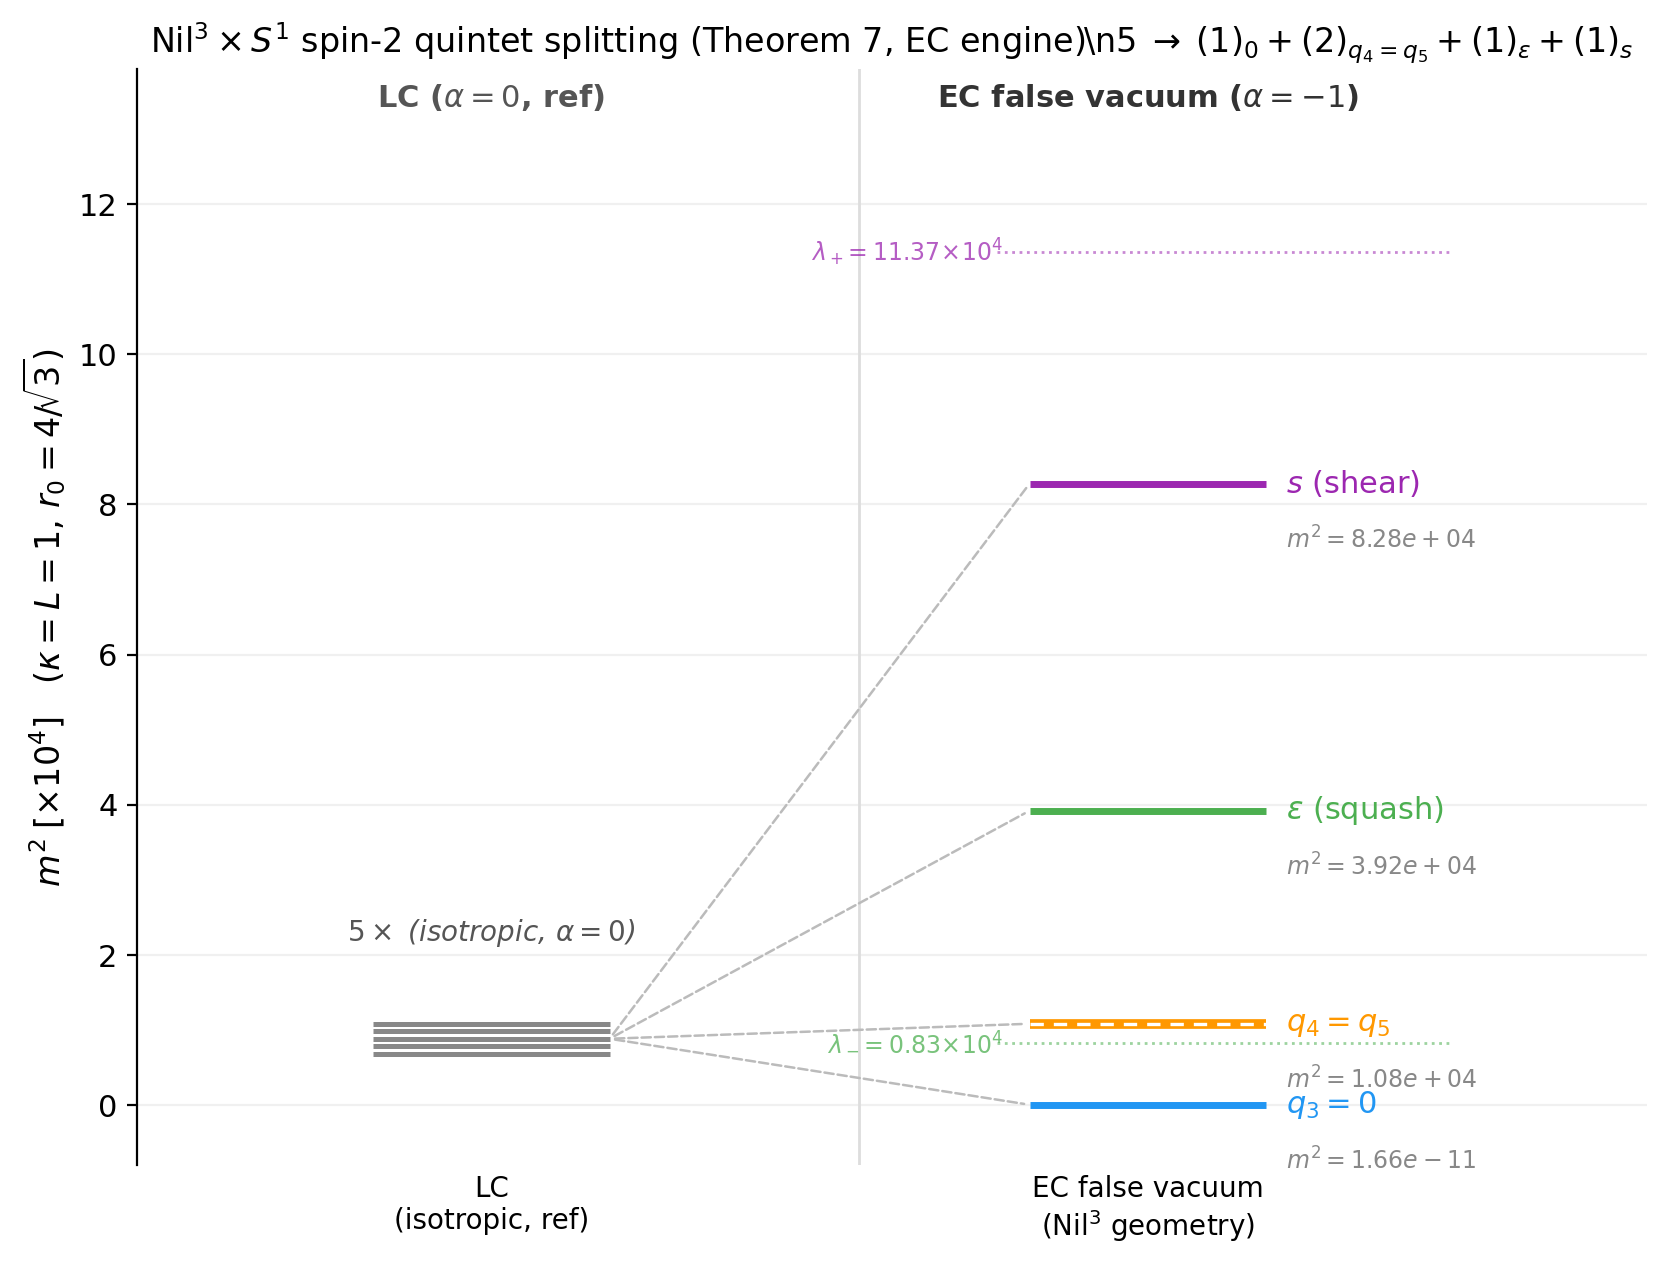
\includegraphics[width=0.9\textwidth]{figures/fig02_nil3_quintet_splitting.png}
  \caption{$\Nilthree$ spin-2 quintet splitting $5\to 0+2+1+1$ at the EC false
    vacuum.  The zero mode $q_3$ is geometrically protected by the
    one-dimensional Lie structure of $\Nilthree$, and the $q_4$--$q_5$ degeneracy
    reflects the symmetric role of $e^0$ and $e^1$ with respect to $C^2_{01}$.}
  \label{fig:quintet}
\end{figure}

\paragraph{Geometric interpretation of $q_3=0$.}
The $G_3$ transformation is a hyperbolic rotation in the $(e^0,e^1)$ plane:
\begin{equation}
  e^0 \to c_3 e^0 + s_3 e^1,
  \quad
  e^1 \to s_3 e^0 + c_3 e^1
  \quad (c_3^2 - s_3^2 = 1).
\end{equation}
Under this transformation, the sole structure constant $C^2_{01}$ transforms as
\begin{equation}
  C^2_{01} \to \frac{c_3^2 - s_3^2}{R} = \frac{1}{R}
\end{equation}
(hyperbolic identity), and is therefore invariant.  Consequently $\Veff$ has no
$q_3$ dependence and $m^2(q_3)=0$.  This is a geometric symmetry protection
by the one-dimensional Lie structure of $\Nilthree$ ($C^2_{01}$ only), not a
tachyonic instability.

\paragraph{Interpretation of $q_4=q_5$ degeneracy.}
$G_4$ and $G_5$ are hyperbolic rotations in the $(0\text{--}2)$ and
$(1\text{--}2)$ planes, respectively.  In $\Nilthree$, $e^2$ is the ``result
axis'' of $C^2_{01}$, and $e^0, e^1$ play symmetric roles with respect to
$C^2_{01}$.  This symmetry forces $m^2(q_4)=m^2(q_5)$.

Script: \texttt{paper03ec/nil3\_spin2\_quintet\_splitting.py}.

\subsection{Theorem~8: Uniaxial Mass Splitting}
\label{sec:nil3:thm8}

\begin{theorem}[Uniaxial mass splitting]\label{thm:uniaxial}
  In the spin-1 sector of $\Nilthree\times\Sone$, only one axis acquires a
  mass via the directional selectivity of $C^2_{01}$\textup{:}
  \begin{equation}
    m^2(\omega_2) = \frac{24\pi^4 L^3 R^2 - 256\pi^4 L^3\alpha\kappa^2}{3R^3\kappa^2}
    \neq 0,
    \qquad
    m^2(\omega_0) = m^2(\omega_1) = 0.
  \end{equation}
  At the EC false vacuum $r_0 = 4\kappa a/\sqrt{3}$ ($\alpha=-a^2$)\textup{:}
  \begin{equation}
    m^2(\omega_2)\big|_{r_0} = \frac{6\sqrt{3}\,\pi^4 L^3}{a\kappa^3}.
  \end{equation}
\end{theorem}

\paragraph{Physical interpretation.}
$C^2_{01}$ corresponds to the non-commutativity in the $(0\text{--}1)$ plane
direction.  $\omega_2$ is the twist in the $(0\text{--}1)$ direction, and only
this component acquires a mass from $C^2_{01}\neq 0$.  $\omega_0$ and $\omega_1$
are commutative directions (with respect to $C^2_{01}$) and remain massless.
This structure is termed uniaxial mass splitting.  The one-dimensional Lie
algebra structure of $\Nilthree$ ($C^2_{01}$ only non-zero) gives mass to the
unique $\omega_2$ among the spin-1 triplet, while keeping the other two
massless.

\subsection{EFT around the $\Nilthree$ EC False Vacuum}
\label{sec:nil3:eft}

We determine the quadratic effective action around the EC false vacuum
$r_0=4\kappa a/\sqrt{3}$.

\paragraph{Full quadratic coefficient spectrum (numerical values at $a=\kappa=L=1$).}

\begin{table}[H]
\centering
\resizebox{\linewidth}{!}{%
\begin{tabular}{llll}
\toprule
DOF & Quadratic coefficient (analytic) & Numeric ($a=\kappa=L=1$) & $\alpha$-dependence \\
\midrule
$r$ (radial) & $2\sqrt{3}\pi^4 L/(a\kappa^3)$ & 337.4 & $\propto 1/a$ (light) \\
$\omega_2$ (non-comm.\ spin-1) & $6\sqrt{3}\pi^4 L^3/(a\kappa^3)$ & 1012 & $\propto 1/a$ (light) \\
$\eta$ (axial torsion; non-prop.) & $128\sqrt{3}\pi^4 La/\kappa$ & 21,596 & $\propto a$ (heavy) \\
spin-2 squash $\varepsilon$ & $6272\sqrt{3}\pi^4 La/(27\kappa)$ & 39,192 & $\propto a$ (heavy) \\
$\omega_0,\omega_1$ & $0$ & 0 & massless \\
$q_3$ (zero mode) & $0$ & 0 & zero mode \\
$q_4,q_5$ & $m^2(q_4)=m^2(q_5)$ & 10,798 & --- \\
\bottomrule
\end{tabular}%
}
\caption{Quadratic coefficient spectrum of the $\Nilthree$ EC false-vacuum EFT
  at $a=\kappa=L=1$.  The $\eta$ row gives the potential curvature in the $\eta$
  direction under Palatini protection ($G_{\eta\eta}=0$), not a propagating mass.}
\label{tab:nil3eft}
\end{table}

\paragraph{Two-group hierarchy.}
``Geometric modes'' ($r$, $\omega_2$) scale as $\propto 1/a$ (lighter for
large $|\alpha|$), while ``torsion/curvature modes'' ($\eta$-direction curvature,
spin-2) scale as $\propto a$ (heavier for large $|\alpha|$).

The quadratic effective action is
\begin{equation}
\begin{aligned}
  \Veff^{Nil^3}_\mathrm{EFT}(\delta\Phi)
  &\approx V_0 + \frac{1}{2}\Bigg[
    \frac{2\sqrt{3}\pi^4 L}{a\kappa^3}(\delta r)^2
    + \frac{128\sqrt{3}\pi^4 La}{\kappa}(\delta\eta)^2 \\
  &\quad
    + \frac{6272\sqrt{3}\pi^4 La}{27\kappa}(\delta\varepsilon)^2
    + \frac{6\sqrt{3}\pi^4 L^3}{a\kappa^3}(\delta\omega_2)^2
  \Bigg]
  + O(\delta^3)
\end{aligned}
\end{equation}
with the cross-term $\partial^2 V/\partial r\partial\eta|_{r_0,0}=0$.
Scripts: \texttt{paper03ec/nil3\_false\_vacuum\_eft.py}.

\subsection{Mode Dictionary Table ($\Nilthree\times\Sone$)}
\label{sec:nil3:table}

\begin{table}[H]
\centering
\resizebox{\linewidth}{!}{%
\begin{tabular}{lccc}
\toprule
Quantity & AX ($V=0,\,\eta\neq 0$) & VT ($\eta=0,\,V\neq 0$) & EC false vac.\ ($\eta=V=0$, $\alpha<0$) \\
\midrule
$C^2_\EC$ & $4/(3R^4)$ & $4/(3R^4)$ & $4/(3R^4)$ \\
AX/VT dropout & \checkmark & \checkmark & $\times$ ($C^2_\LC\neq 0$) \\
spin-0: $r$ & propagating & propagating & prop., $m^2_r = 2\sqrt{3}\pi^4 L/(a\kappa^3)$ \\
spin-0: $\eta,V$ & $\eta$ non-prop. & $V$ non-prop. & $\eta$ non-prop.; curvature coeff.\ $= 128\sqrt{3}\pi^4 La/\kappa$ \\
spin-2 $\mu^2$ & $(1056\pi^4 LR^2-19456\pi^4 L\alpha\kappa^2)/(27R\kappa^2)$ & same & at $r_0$: $6272\sqrt{3}\pi^4 La/(27\kappa)$ \\
spin-2 splitting & (isotropic pt.) & --- & $5\to 0+2+1+1$ (Thm.~7) \\
spin-1 splitting & $m^2(\omega_2)\neq 0$, $m^2(\omega_{0,1})=0$ (Thm.~8) & --- & $m^2(\omega_2)=6\sqrt{3}\pi^4 L^3/(a\kappa^3)$ \\
\bottomrule
\end{tabular}%
}
\caption{$\Nilthree\times\Sone$ mode dictionary under EC--Weyl.}
\label{tab:nil3}
\end{table}

\paragraph{Supplementary note on the $\Nilthree$ MX background.}
In the MX background ($V\neq 0,\eta\neq 0$), the general formula of
\S\ref{sec:ecweyl:mx} gives
\begin{equation}
  \Delta\Veff^{\EC}(\Nilthree, \mathrm{MX})
  = -\frac{256\pi^4 LRV^2\alpha\eta^2}{3} \neq 0
\end{equation}
as the EC--LC difference (SymPy: \texttt{nil3\_mode\_dictionary.py}).
However, the MX stationarity conditions ($\theta_\NY=0$):
\begin{equation}
  V_* = \pm\frac{3}{4}\sqrt{\frac{1}{\alpha}},
  \qquad
  \eta_* = \pm\frac{R}{4}\sqrt{\frac{1}{\alpha}},
\end{equation}
are purely imaginary for $\alpha<0$ (no real MX stationary point).  Numerical
root search by \texttt{paper03ec/nil3\_mx\_vacuum\_search.py} finds no MX stable
point for general $\theta_\NY$ either; the only local minimum remaining is the
$\eta=V=0$ false vacuum.  The EC-specific physics of $\Nilthree$ (false vacuum,
quintet splitting) originates from $C^2_\LC\neq 0$ on the $\eta=V=0$ section,
independently of the MX correction.
